\documentclass[conference]{IEEEtran}
\IEEEoverridecommandlockouts

\usepackage{cite}
\usepackage{amsmath,amssymb,amsfonts}
\usepackage{graphicx}
\usepackage{textcomp}
\usepackage{xcolor}

\begin{document}

\title{Validated Extension of a 2-D Reflector Model to Sinusoidal Open Strips}

\author{
\IEEEauthorblockN{Author Name}
\IEEEauthorblockA{
\textit{Affiliation} \\
City, Country \\
email@example.com
}
}

\maketitle

\begin{abstract}
This paper presents a verified numerical extension of a two-dimensional E-wave reflector model based on the method of discrete singularities and complex-source-point excitation. The baseline implementation is first validated against the canonical parabolic-reflector study of Nosich and Gandel. For the benchmark case with aperture equal to thirty wavelengths, focal length equal to one half of the aperture, and beam parameter equal to 2.5, the computed solution gives a machine-level boundary residual, broadside radiation, and symmetric edge illumination of about ten decibels, in agreement with the published rule for optimum performance. The validated solver is then extended to open sinusoidal strips parameterized by length, amplitude, and spatial frequency. A compact sweep shows that the strip geometry strongly controls near-field concentration, with a distinct high-response region appearing for large amplitudes and spatial frequencies around 0.2 cycles per wavelength. The study therefore supports the use of the validated reflector model as a practical tool for exploring nonclassical quasioptical reflector shapes.
\end{abstract}

\begin{IEEEkeywords}
reflector antennas, method of discrete singularities, complex source point, near-field modeling, sinusoidal strip
\end{IEEEkeywords}

\section{Introduction}
Two-dimensional quasioptical reflector models remain attractive whenever high-frequency asymptotics are not accurate enough and a full-wave solution is still required. A particularly efficient formulation for electrically large perfectly conducting open reflectors was given in \cite{nosich2007}, where the method of discrete singularities (MDS) was combined with a complex-source-point (CSP) feed model to analyze single and multireflector antennas in the E-wave case. That paper is a strong benchmark because it links the integral-equation formulation, the CSP excitation, and the well-known empirical rule that the best reflector performance is obtained for edge illumination close to ten decibels.

For a short ICTON-style contribution, an incremental paper is acceptable only if the contribution is stated honestly. In the present work, the contribution is not a new integral equation. Instead, it is a validated implementation of the MDS/CSP reflector model and its extension to a new reflector family: open sinusoidal strips. The goal is to answer a simple design question: how do sinusoidal-strip amplitude and spatial frequency modify the near-field concentration produced by a beam-like feed?

This framing is useful for two reasons. First, the sinusoidal strip is clearly outside the canonical reflector shapes treated in \cite{nosich2007}. Second, the extension can be studied with the same solver infrastructure once the contour parameterization is generalized. The paper is therefore organized as follows. Section~II summarizes the formulation used in the present implementation and validates it against the parabolic benchmark from \cite{nosich2007}. Section~III introduces the sinusoidal-strip extension and reports a compact parametric study. Section~IV concludes the paper and outlines the most promising next steps.

\section{Formulation and Validation}
The continuous model follows the E-wave reflector-scattering formulation in \cite{nosich2007}. Reflectors are treated as zero-thickness perfectly conducting open strips. The primary feed is represented by a CSP beam, which is a standard way to emulate a directive horn-like source in two-dimensional reflector analysis \cite{deschamps1971,oguzer2002}. In the implementation used here, all lengths are normalized by the wavelength, so that $k = 2\pi$.

The main extension required for the present study is geometric rather than analytical. The solver accepts any open contour that can be parameterized as
\begin{equation}
\Gamma = \{(x(t),y(t)):\; -1 \le t \le 1\},
\end{equation}
with numerically accessible first derivatives. This makes it possible to retain the validated MDS/CSP workflow while replacing the reflector geometry.

For the sinusoidal-strip extension, the open contour is defined by
\begin{equation}
\Gamma_{s} = \left\{(x,y):\;
y = y_{b} + A \sin \left[ 2\pi \nu (x-x_{c}) + \phi \right],\;
x_{c}-\frac{L}{2} \le x \le x_{c}+\frac{L}{2}
\right\},
\label{eq:strip}
\end{equation}
where $L$ is the strip length, $A$ is the oscillation amplitude, $\nu$ is the spatial frequency in cycles per wavelength, and $\phi$ is the phase shift. In the strip scene, the CSP beam is pointed automatically to a chosen point on the strip,
\begin{equation}
\beta = \operatorname{atan2}(y_{t}-y_{0},\,x_{t}-x_{0}),
\label{eq:beta}
\end{equation}
so that the excitation remains physically consistent when the strip parameters are changed.

Before using \eqref{eq:strip} in a new study, the implementation must be anchored to a published result. We therefore reproduced the single parabolic benchmark from \cite{nosich2007}, using aperture $d=30\lambda$, focal length $f=0.5d$, and CSP beam parameter $kb=2.5$. The resulting near field is shown in Fig.~\ref{fig:baseline}, and the numerical indicators are summarized in Table~\ref{tab:validation}.

\begin{figure}[t]
\centering
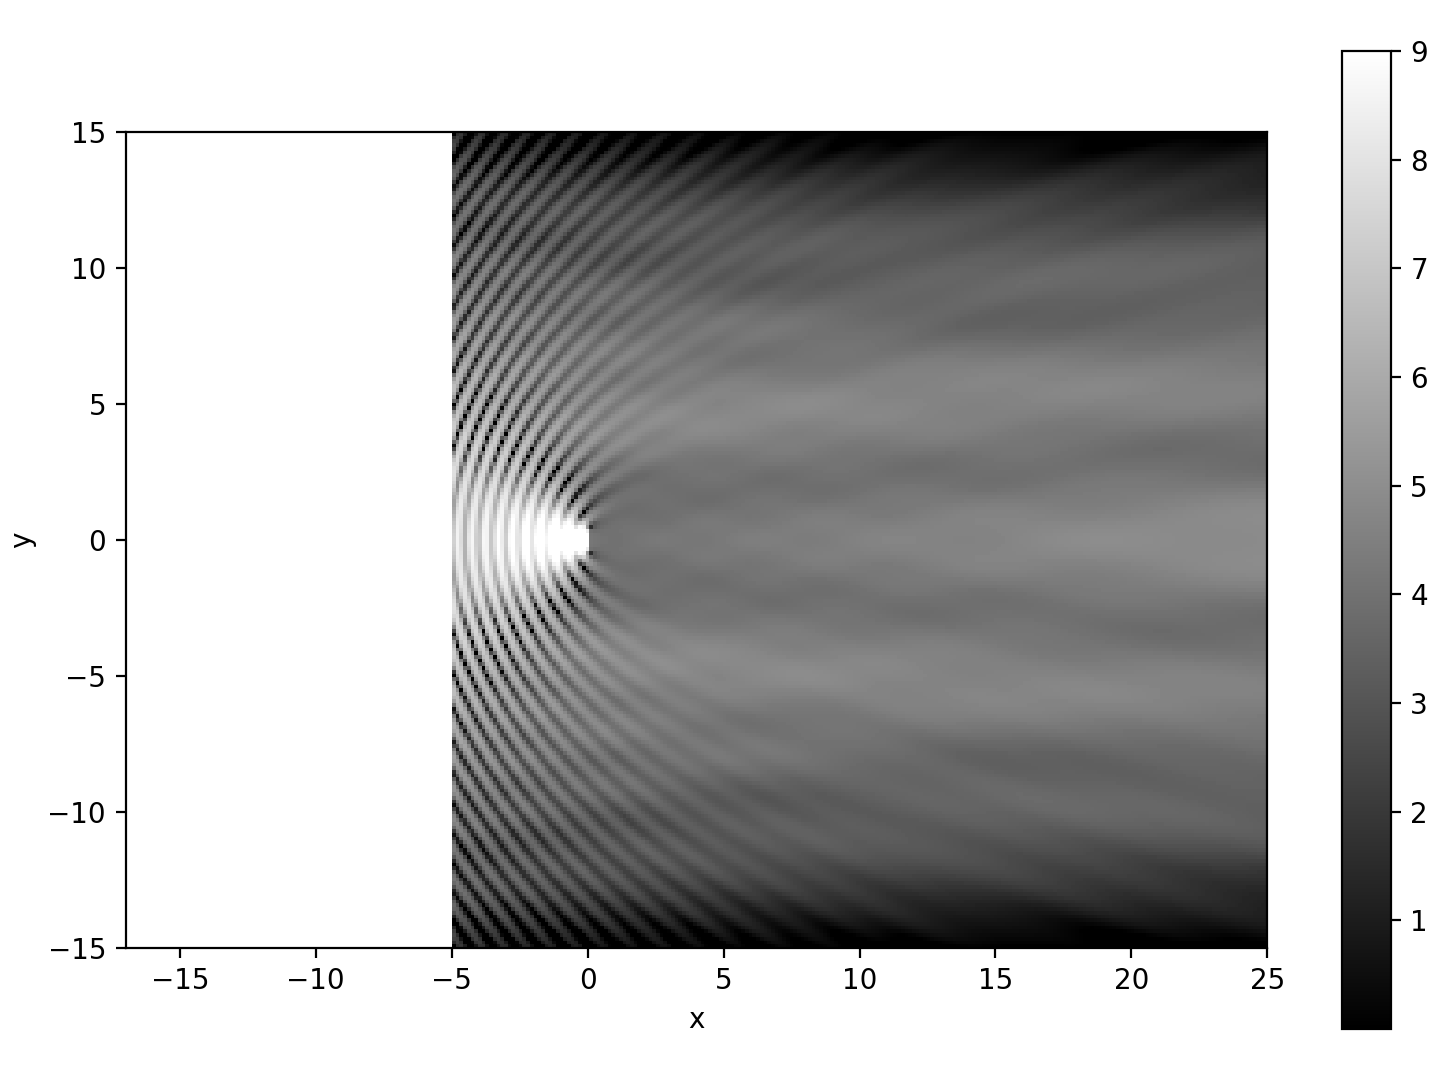
\includegraphics[width=0.95\columnwidth]{baseline_parabola_total_near.png}
\caption{Validated single-parabolic-reflector benchmark used to anchor the extension study. Parameters: $d=30\lambda$, $f=0.5d$, and $kb=2.5$.}
\label{fig:baseline}
\end{figure}

\begin{table}[t]
\caption{Validation summary for the parabolic benchmark.}
\label{tab:validation}
\centering
\footnotesize
\begin{tabular}{|l|c|}
\hline
Quantity & Value \\
\hline
Reflector aperture $d$ & $30\lambda$ \\
Focal length $f$ & $0.5d$ \\
CSP beam parameter $kb$ & 2.5 \\
Peak radiation angle & $0^\circ$ \\
Edge illumination (left/right) & $-9.65$ dB / $-9.65$ dB \\
Boundary residual & $1.06\times10^{-15}$ \\
Computed directivity & 72.68 \\
\hline
\end{tabular}
\end{table}

The most important observation is not the directivity itself but the edge illumination. The computed value of $-9.65$ dB reproduces the ten-decibel optimum discussed in \cite{nosich2007}. Together with the machine-level residual and the correct broadside main beam, this gives enough confidence to use the same implementation as the baseline for a geometry extension study.

\section{Sinusoidal-Strip Extension}
The sinusoidal-strip scene was built as a single open reflector placed near the bottom of the computational window. Unless noted otherwise, the strip baseline is $y_{b}=-10\lambda$, the strip center is at $x_{c}=0$, the phase in \eqref{eq:strip} is zero, and the CSP beam parameter is $kb=9$. The feed is placed above the strip and aimed at its midpoint by \eqref{eq:beta}. The resulting geometry is simple, but it is rich enough to test whether a validated reflector solver can identify nontrivial near-field trends for noncanonical reflectors.

To quantify the extension, we used the scattered field only and defined the central observation metric
\begin{equation}
Q(A,\nu) = \max_{(x,y)\in\Omega_{c}} \left|u^{\mathrm{sc}}(x,y)\right|^{2},
\label{eq:qmetric}
\end{equation}
with
\begin{equation}
\Omega_{c} = [-6,6]\times[-8.5,-3]\;\lambda.
\end{equation}
This window excludes the direct feed hotspot and suppresses the strongest strip-end singularities, so the metric focuses on the central near-field response of the sinusoidal reflector itself.

We then swept
\[
A \in \{0.5,\,1.0,\,1.5,\,2.0,\,2.5\}\lambda
\]
and
\[
\nu \in \{0.10,\,0.15,\,0.20,\,0.25,\,0.30\}\;\lambda^{-1},
\]
with a fixed strip length of $L=24\lambda$. All presented strip cases remained numerically stable, with boundary residuals below $5.2\times10^{-12}$.

\begin{figure*}[t]
\centering
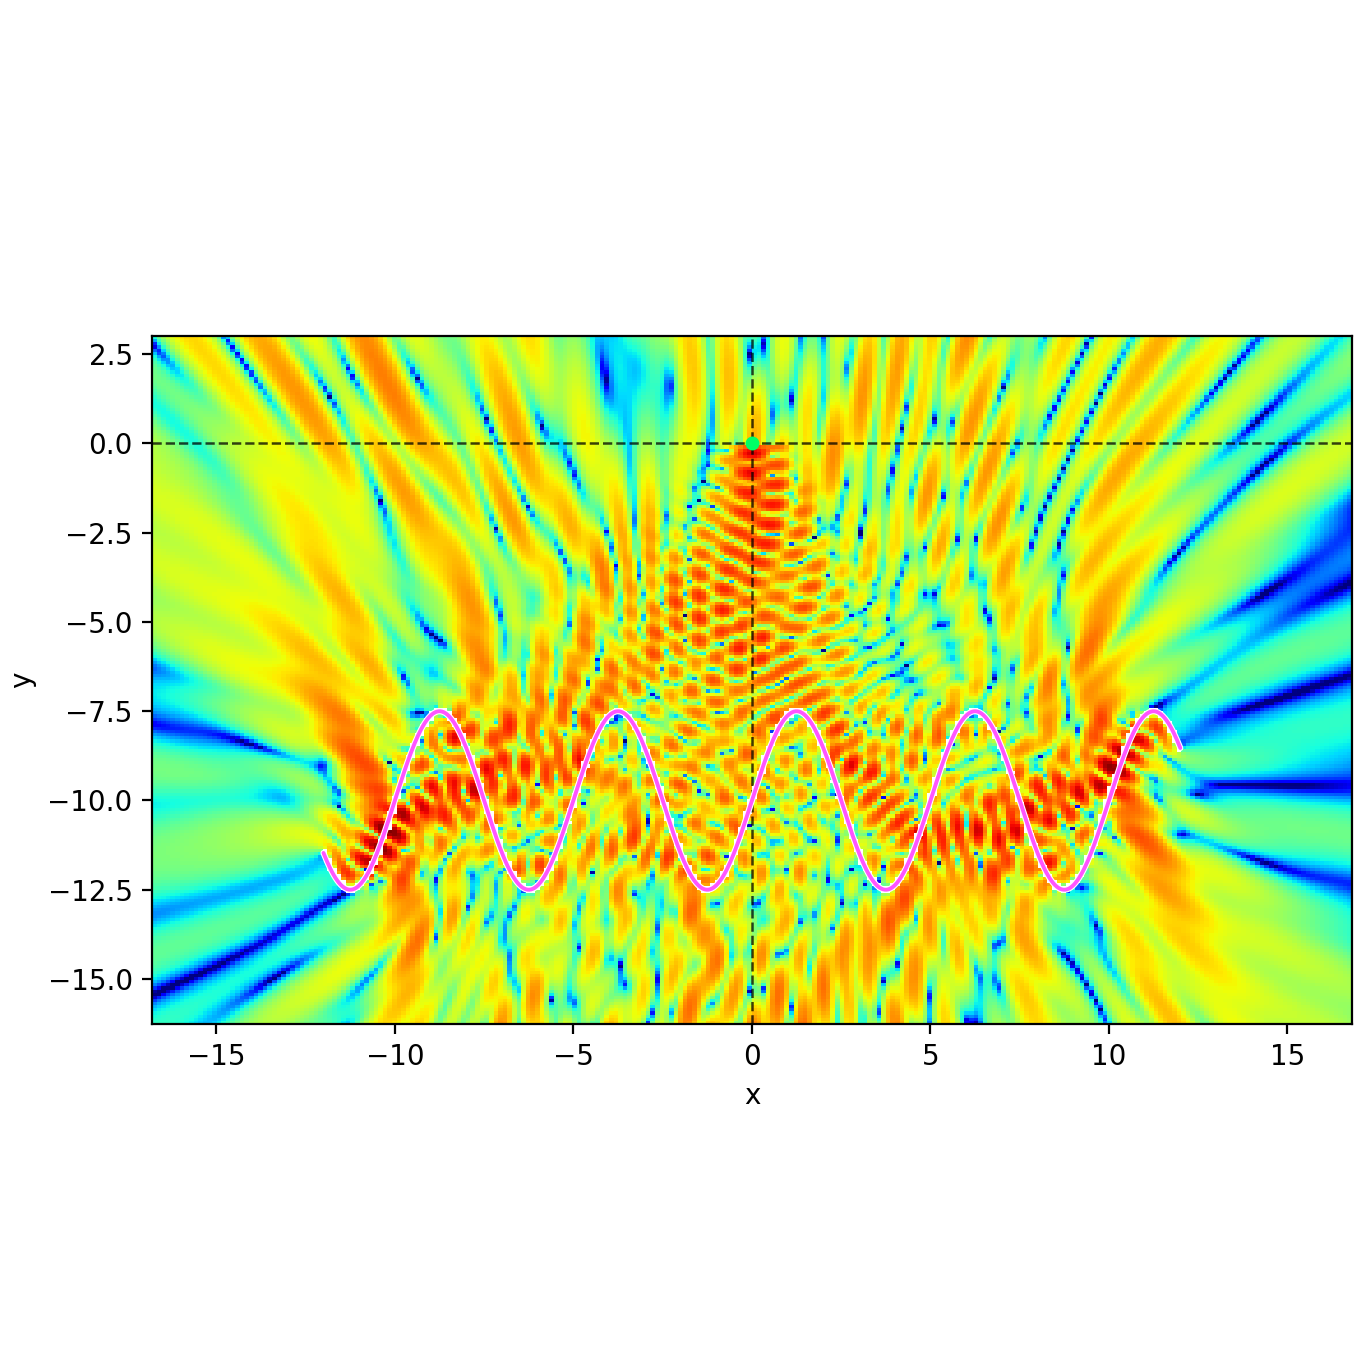
\includegraphics[width=0.72\textwidth]{sinusoidal_bestcase_total_near.png}
\caption{Representative total near field for the sinusoidal-strip extension. Parameters: $L=24\lambda$, $A=2.5\lambda$, $\nu=0.20\,\lambda^{-1}$, $\phi=0$, and $kb=9$. The CSP beam is aimed at the strip midpoint.}
\label{fig:stripfield}
\end{figure*}

\begin{figure}[t]
\centering
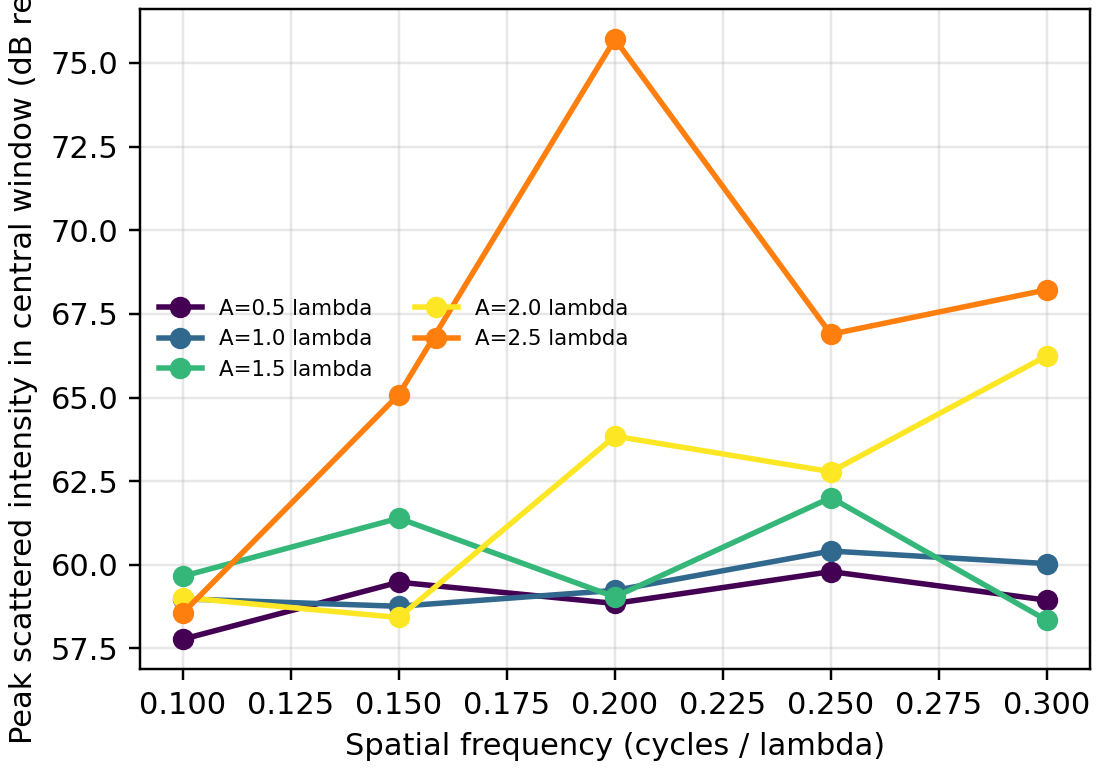
\includegraphics[width=\columnwidth]{sinusoidal_metric_lines.png}
\caption{Peak scattered intensity in the central observation window versus strip spatial frequency for several amplitudes.}
\label{fig:striplines}
\end{figure}

The response trends are shown in Fig.~\ref{fig:striplines}. Two points are immediately visible. First, weakly modulated strips with $A \le 1.5\lambda$ show only modest variation with frequency. Their central-window peak intensity remains within a relatively narrow band, which suggests that the strip behaves as a gently perturbed open reflector rather than a strongly shaping surface. Second, once the amplitude reaches $2.0\lambda$ and above, the response becomes sharply nonmonotonic. This is especially clear for $A=2.5\lambda$, where the best tested case appears at $\nu=0.20\,\lambda^{-1}$.

Using the metric in \eqref{eq:qmetric}, the configuration $A=2.5\lambda$ and $\nu=0.20\,\lambda^{-1}$ produced the strongest central-window response in the tested set. Relative to the weakly modulated reference case $A=0.5\lambda$ and $\nu=0.10\,\lambda^{-1}$, the increase in $Q$ is about 18 dB. The corresponding field map in Fig.~\ref{fig:stripfield} shows why. The strip does not create a single classical geometrical focus in the same sense as an ellipse. Instead, it behaves as a distributed corrugated reflector that redistributes the beam energy and creates strong localized near-field regions around selected parts of the sinusoidal contour.

This observation is scientifically useful because it refines the original extension claim. The sinusoidal strip is better interpreted as a beam-shaping and near-field-localization element than as a direct replacement for a classical single-focus reflector. That is still a meaningful extension for ICTON-type topics because the same validated full-wave model can now be used to explore nonstandard surfaces for near-field engineering.

\section{Conclusion}
This paper reported a validated extension of a two-dimensional MDS/CSP reflector model to open sinusoidal strips. The implementation was first anchored to the canonical parabolic benchmark of \cite{nosich2007}, where it reproduced the expected broadside behavior and the published ten-decibel edge-illumination rule with a residual close to machine precision. The same solver was then applied to a compact sinusoidal-strip study with amplitude and spatial frequency as the main design variables.

The extension results show that sinusoidal modulation can change the near-field response dramatically. For weak modulation, the scattered-field concentration varies only mildly with frequency. For larger amplitudes, however, a sharp high-response region appears, with the strongest tested case at $A=2.5\lambda$ and $\nu=0.20\,\lambda^{-1}$. In other words, the validated reflector model is not limited to classical parabolic or elliptic shapes; it can also be used as a fast exploratory platform for noncanonical open reflectors.

The present study is intentionally compact. The next logical steps are a denser parametric sweep, alternative feed placements, a direct comparison with elliptic arcs, and the introduction of optimization targets such as focal spot width or energy concentration inside a prescribed near-field region.

\section*{References}
\begin{thebibliography}{00}
\bibitem{nosich2007}
A. A. Nosich and Y. V. Gandel, ``Numerical analysis of quasioptical multireflector antennas in 2-D with the method of discrete singularities: E-wave case,'' \emph{IEEE Transactions on Antennas and Propagation}, vol. 55, no. 2, pp. 399--406, Feb. 2007, doi: 10.1109/TAP.2006.889811.

\bibitem{oguzer2002}
T. O\u{g}uzer, A. I. Nosich, and A. Alt\i nta\c{s}, ``Radiation characteristics of a 2D parabolic reflector antenna excited by the H-polarized complex source,'' in \emph{Proc. Mathematical Methods in Electromagnetic Theory}, 2002, doi: 10.1109/MMET.2002.1107026.

\bibitem{deschamps1971}
G. A. Deschamps, ``Gaussian beam as a bundle of complex rays,'' \emph{Electronics Letters}, vol. 7, no. 23, pp. 684--685, 1971, doi: 10.1049/el:19710467.

\bibitem{josa2007}
A. A. Nosich, Y. V. Gandel, T. Magath, and A. Altintas, ``Numerical analysis and synthesis of 2-D quasioptical reflectors and beam waveguides based on an integral-equation approach with Nystrom's discretization,'' \emph{Journal of the Optical Society of America A}, vol. 24, no. 9, pp. 2831--2836, 2007.
\end{thebibliography}

\end{document}
